\documentclass[]{article}
\usepackage{lmodern}
\usepackage{amssymb,amsmath}
\usepackage{ifxetex,ifluatex}
\usepackage{fixltx2e} % provides \textsubscript
\ifnum 0\ifxetex 1\fi\ifluatex 1\fi=0 % if pdftex
  \usepackage[T1]{fontenc}
  \usepackage[utf8]{inputenc}
\else % if luatex or xelatex
  \ifxetex
    \usepackage{mathspec}
  \else
    \usepackage{fontspec}
  \fi
  \defaultfontfeatures{Ligatures=TeX,Scale=MatchLowercase}
\fi
% use upquote if available, for straight quotes in verbatim environments
\IfFileExists{upquote.sty}{\usepackage{upquote}}{}
% use microtype if available
\IfFileExists{microtype.sty}{%
\usepackage{microtype}
\UseMicrotypeSet[protrusion]{basicmath} % disable protrusion for tt fonts
}{}
\usepackage[margin=1in]{geometry}
\usepackage{hyperref}
\hypersetup{unicode=true,
            pdftitle={Assignment 5, speach recognition},
            pdfauthor={Albert Öst, Per Emil Hammarlund},
            pdfborder={0 0 0},
            breaklinks=true}
\urlstyle{same}  % don't use monospace font for urls
\usepackage{longtable,booktabs}
\usepackage{graphicx,grffile}
\makeatletter
\def\maxwidth{\ifdim\Gin@nat@width>\linewidth\linewidth\else\Gin@nat@width\fi}
\def\maxheight{\ifdim\Gin@nat@height>\textheight\textheight\else\Gin@nat@height\fi}
\makeatother
% Scale images if necessary, so that they will not overflow the page
% margins by default, and it is still possible to overwrite the defaults
% using explicit options in \includegraphics[width, height, ...]{}
\setkeys{Gin}{width=\maxwidth,height=\maxheight,keepaspectratio}
\IfFileExists{parskip.sty}{%
\usepackage{parskip}
}{% else
\setlength{\parindent}{0pt}
\setlength{\parskip}{6pt plus 2pt minus 1pt}
}
\setlength{\emergencystretch}{3em}  % prevent overfull lines
\providecommand{\tightlist}{%
  \setlength{\itemsep}{0pt}\setlength{\parskip}{0pt}}
\setcounter{secnumdepth}{0}
% Redefines (sub)paragraphs to behave more like sections
\ifx\paragraph\undefined\else
\let\oldparagraph\paragraph
\renewcommand{\paragraph}[1]{\oldparagraph{#1}\mbox{}}
\fi
\ifx\subparagraph\undefined\else
\let\oldsubparagraph\subparagraph
\renewcommand{\subparagraph}[1]{\oldsubparagraph{#1}\mbox{}}
\fi

%%% Use protect on footnotes to avoid problems with footnotes in titles
\let\rmarkdownfootnote\footnote%
\def\footnote{\protect\rmarkdownfootnote}

%%% Change title format to be more compact
\usepackage{titling}

% Create subtitle command for use in maketitle
\providecommand{\subtitle}[1]{
  \posttitle{
    \begin{center}\large#1\end{center}
    }
}

\setlength{\droptitle}{-2em}

  \title{Assignment 5, speach recognition}
    \pretitle{\vspace{\droptitle}\centering\huge}
  \posttitle{\par}
    \author{Albert Öst, Per Emil Hammarlund}
    \preauthor{\centering\large\emph}
  \postauthor{\par}
      \predate{\centering\large\emph}
  \postdate{\par}
    \date{5/29/2019}

\usepackage{float}
\let\origfigure\figure
\let\endorigfigure\endfigure
\renewenvironment{figure}[1][2] {
    \expandafter\origfigure\expandafter[H]
} {
    \endorigfigure
}

\begin{document}
\maketitle

\hypertarget{play-example-from-database}{%
\section{Play example from database}\label{play-example-from-database}}

\hypertarget{feature-extraction}{%
\section{Feature extraction}\label{feature-extraction}}

Features where extracted using the provided \(GetSpeachFeatures\), and
the MFCCS from \(GetSpeachFeatures\) was then normalized. The normalized
MFCCS was the feature extracted observation sequence used in the model.

\hypertarget{hmm-design}{%
\section{HMM design}\label{hmm-design}}

\begin{itemize}
\tightlist
\item
  One HMM for each number
\item
  Numbers 0-9
\item
  In each HMM, a hidden state for each phoneme and two silent states
  where added in the beginning and end.
\end{itemize}

\begin{longtable}[]{@{}ll@{}}
\toprule
number & phonemes\tabularnewline
\midrule
\endhead
zero & Z IY R OW\tabularnewline
one & W AH N\tabularnewline
two & T UW\tabularnewline
three & TH R IY\tabularnewline
four & F AO R\tabularnewline
five & F AY V\tabularnewline
six & S IH K S\tabularnewline
seven & S EH V AH N\tabularnewline
eight & EY T\tabularnewline
nine & N AY N\tabularnewline
\bottomrule
\end{longtable}

\begin{itemize}
\tightlist
\item
  To find a good approximation for the initialization of the transition
  prob. matrix. The average numner of time frames for each numbers MFCCS
  (in the train set) was calculated and then divided by the number of
  hidden states. This fraction for each class was then used as the prob.
  of transitioning to the next state.
\end{itemize}

\begin{verbatim}
 avgs =
 
    0.200000000000000
    0.200000000000000
    0.166666666666667
    0.250000000000000
    0.200000000000000
    0.200000000000000
    0.250000000000000
    0.250000000000000
    0.166666666666667
    0.166666666666667
\end{verbatim}

\begin{itemize}
\tightlist
\item
  For example, the first class (zero) was given the following initial
  trans. prob. matrix.
\end{itemize}

\[A_{zero} = \begin{pmatrix}0.8 & 0.2 & 0 & 0 & 0 & 0 & 0\\ 0 & 0.8 & 0.2 & 0 & 0 & 0 & 0 \\ 0 & 0 & 0.8 & 0.2 & 0 & 0  & 0\\ 0 & 0 & 0 & 0.8 & 0.2 & 0 & 0\\ 0 & 0 & 0 & 0 & 0.8 & 0.2 & 0\\0 & 0 & 0 & 0 & 0 & 0.8 & 0.2\end{pmatrix}\]

\begin{itemize}
\item
  All trans. prob. matrices where left-right and finite.
\item
  The emmisions from each hidden state were 13 dimensional vectors. The
  emitters from each hidden state was given a GMM with three components.
\item
  Each of the threee components where given equal mixture coefficients
  \(\pi_i\), a subjectivley non informative diagonal covariance matrix
  (the identity), and the same mean.
\item
  Noise was added to the means and covariances in between hidden states.
\end{itemize}

\hypertarget{training-and-testing-method}{%
\section{Training and testing
method}\label{training-and-testing-method}}

\begin{itemize}
\item
  According to the documentation of
  \href{https://github.com/Jakobovski/free-spoken-digit-dataset}{the
  dataset that we chose}. The test set is is the first 10\% of the
  recordings. So recordings 0-4 in each class and speaker where assigned
  to the test set, and recordings 5-49 where assigned to the training
  set. The HMMs where trained on their respecitve classes using the
  provided \(hmm.train()\) method.
\item
  The HMMs where tested by calculating the log prob for each HMM given
  each observation in the test set. And the accuracy was:
\end{itemize}

\begin{verbatim}
accuracy =

   1.000000000000000
   1.000000000000000
   0.850000000000000
   0.900000000000000
   0.900000000000000
   1.000000000000000
   0.800000000000000
   1.000000000000000
   0.700000000000000
   0.950000000000000
\end{verbatim}

\begin{itemize}
\item
  So all classes had great accuracy except for the number eight. Looking
  at eight, we saw that perhaps three GMM components in the first
  non-silent hidden state seemed to only have two peaks, so we tried to
  use one less component in the GMM. This did not have any effect.
\item
  Furthermore, a few recordings did not pronounce all phonemes. So a
  setup with one less hidden state was tried, but there was no
  significant difference.
\end{itemize}

\newpage

\hypertarget{training-data-vs-randomized-from-hmm}{%
\section{Training data vs randomized from
HMM}\label{training-data-vs-randomized-from-hmm}}

The training data and randomized sequences from the hmms took the
following form.

\begin{figure}
\centering
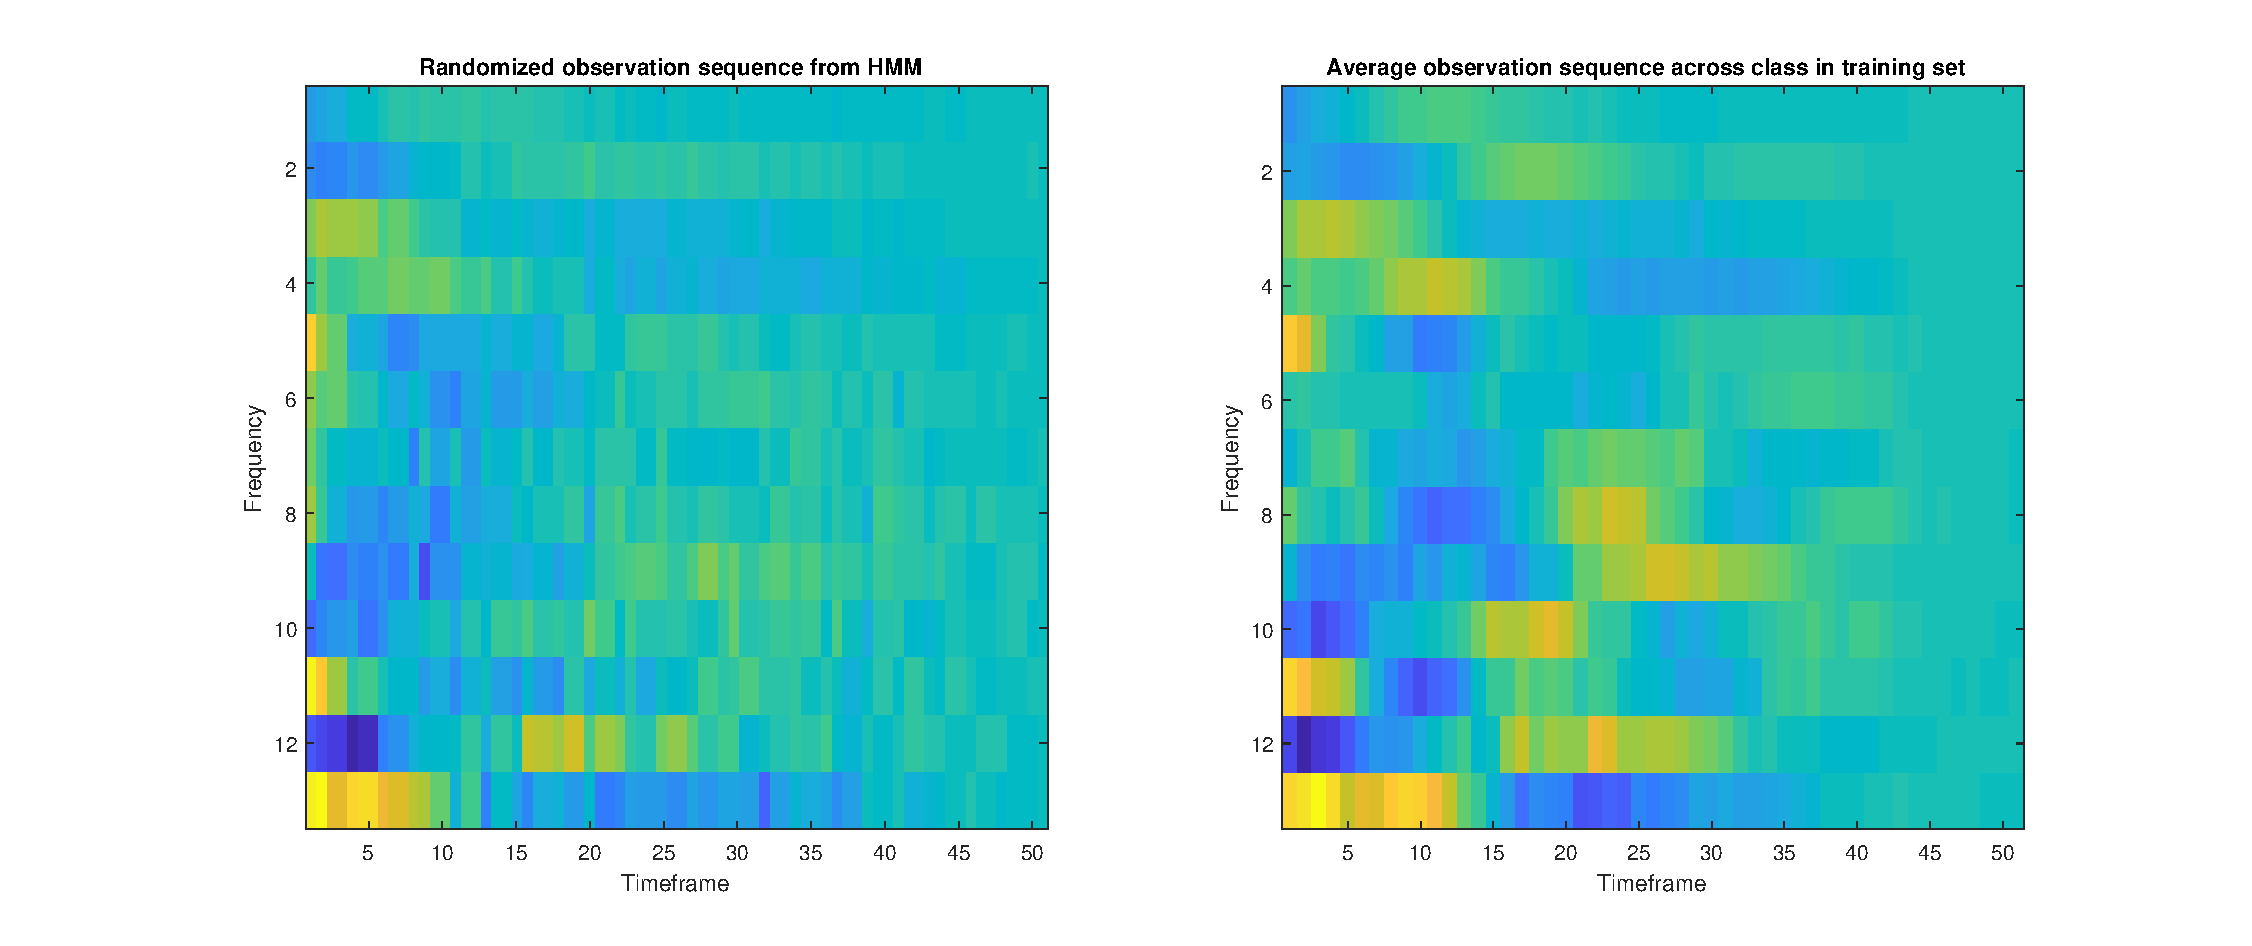
\includegraphics{../Results/randCompClass0.eps}
\caption{Randomized vs training data class zero}
\end{figure}

\begin{figure}
\centering
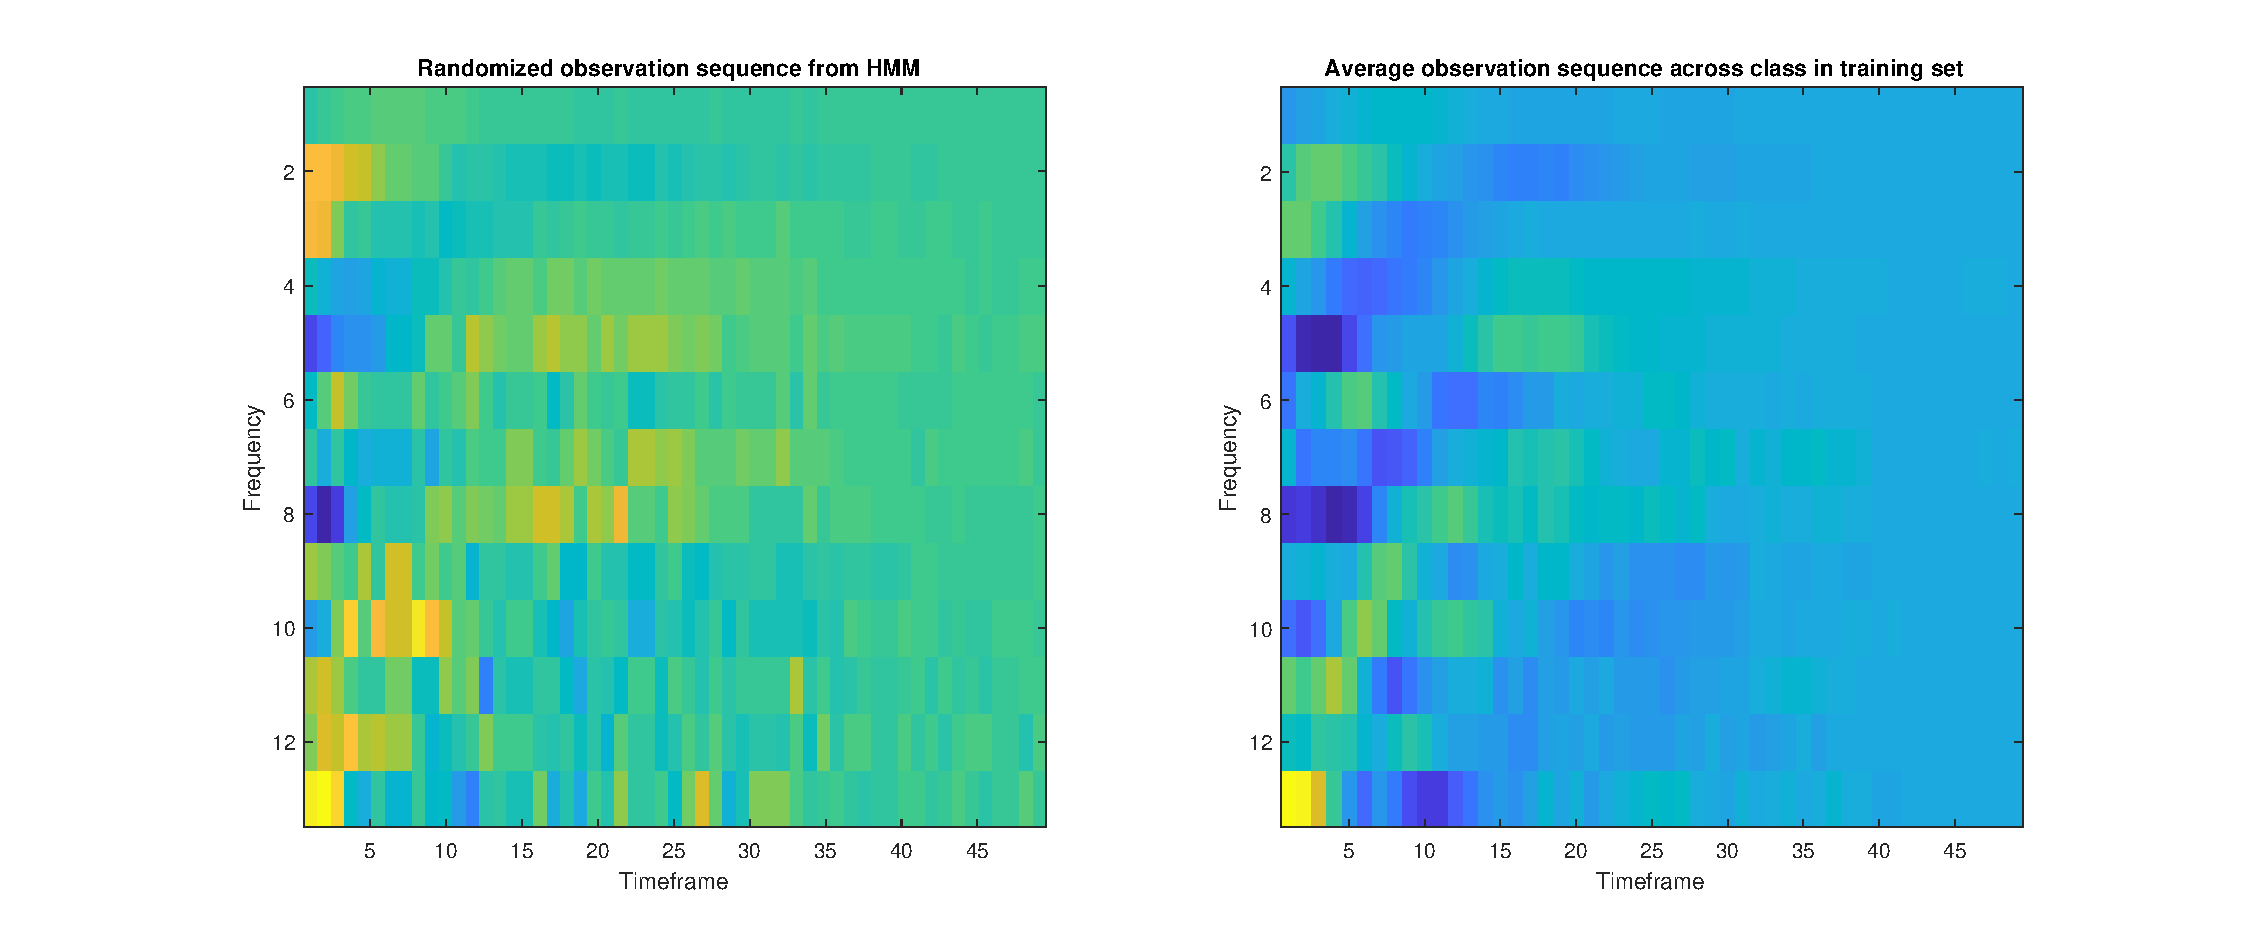
\includegraphics{../Results/randCompClass1.eps}
\caption{Randomized vs training data class one}
\end{figure}

\begin{figure}
\centering
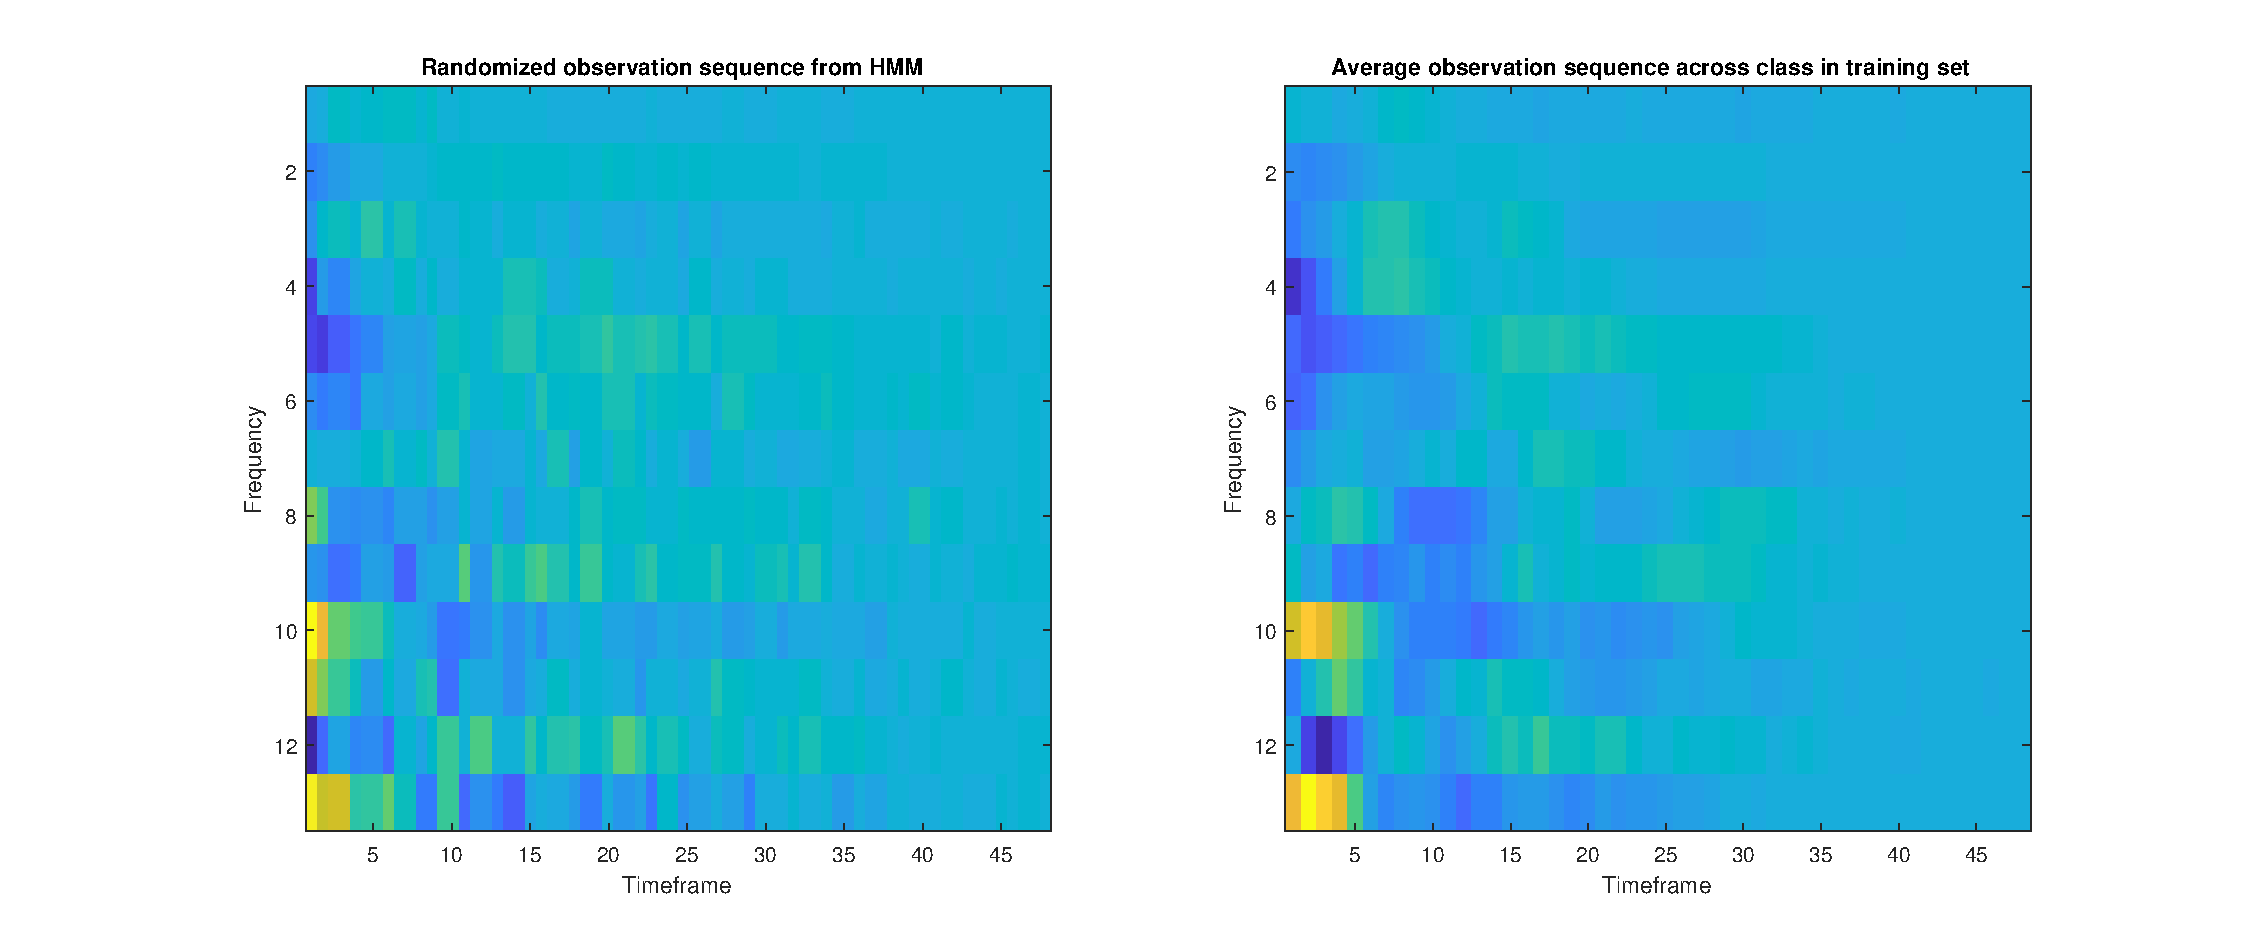
\includegraphics{../Results/randCompClass2.eps}
\caption{Randomized vs training data class two}
\end{figure}

\begin{figure}
\centering
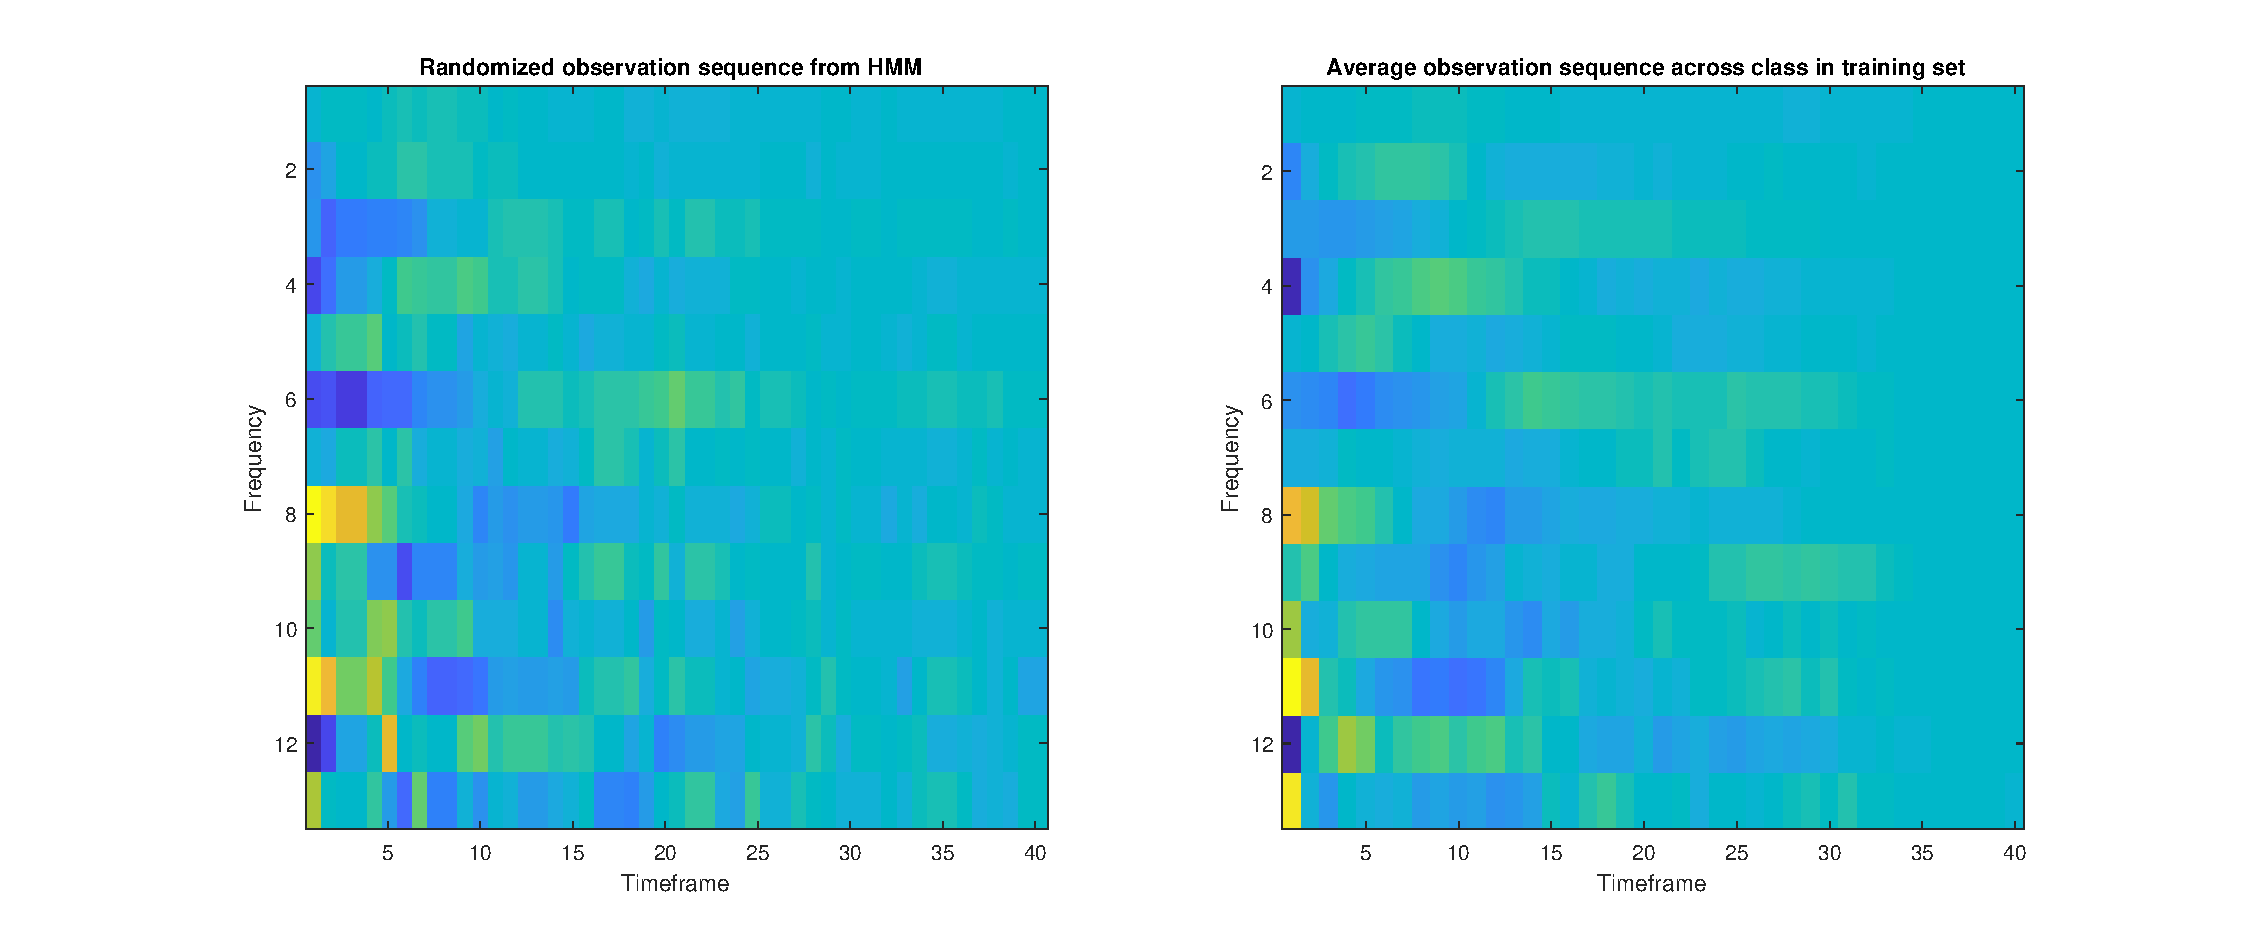
\includegraphics{../Results/randCompClass3.eps}
\caption{Randomized vs training data class three}
\end{figure}

\begin{figure}
\centering
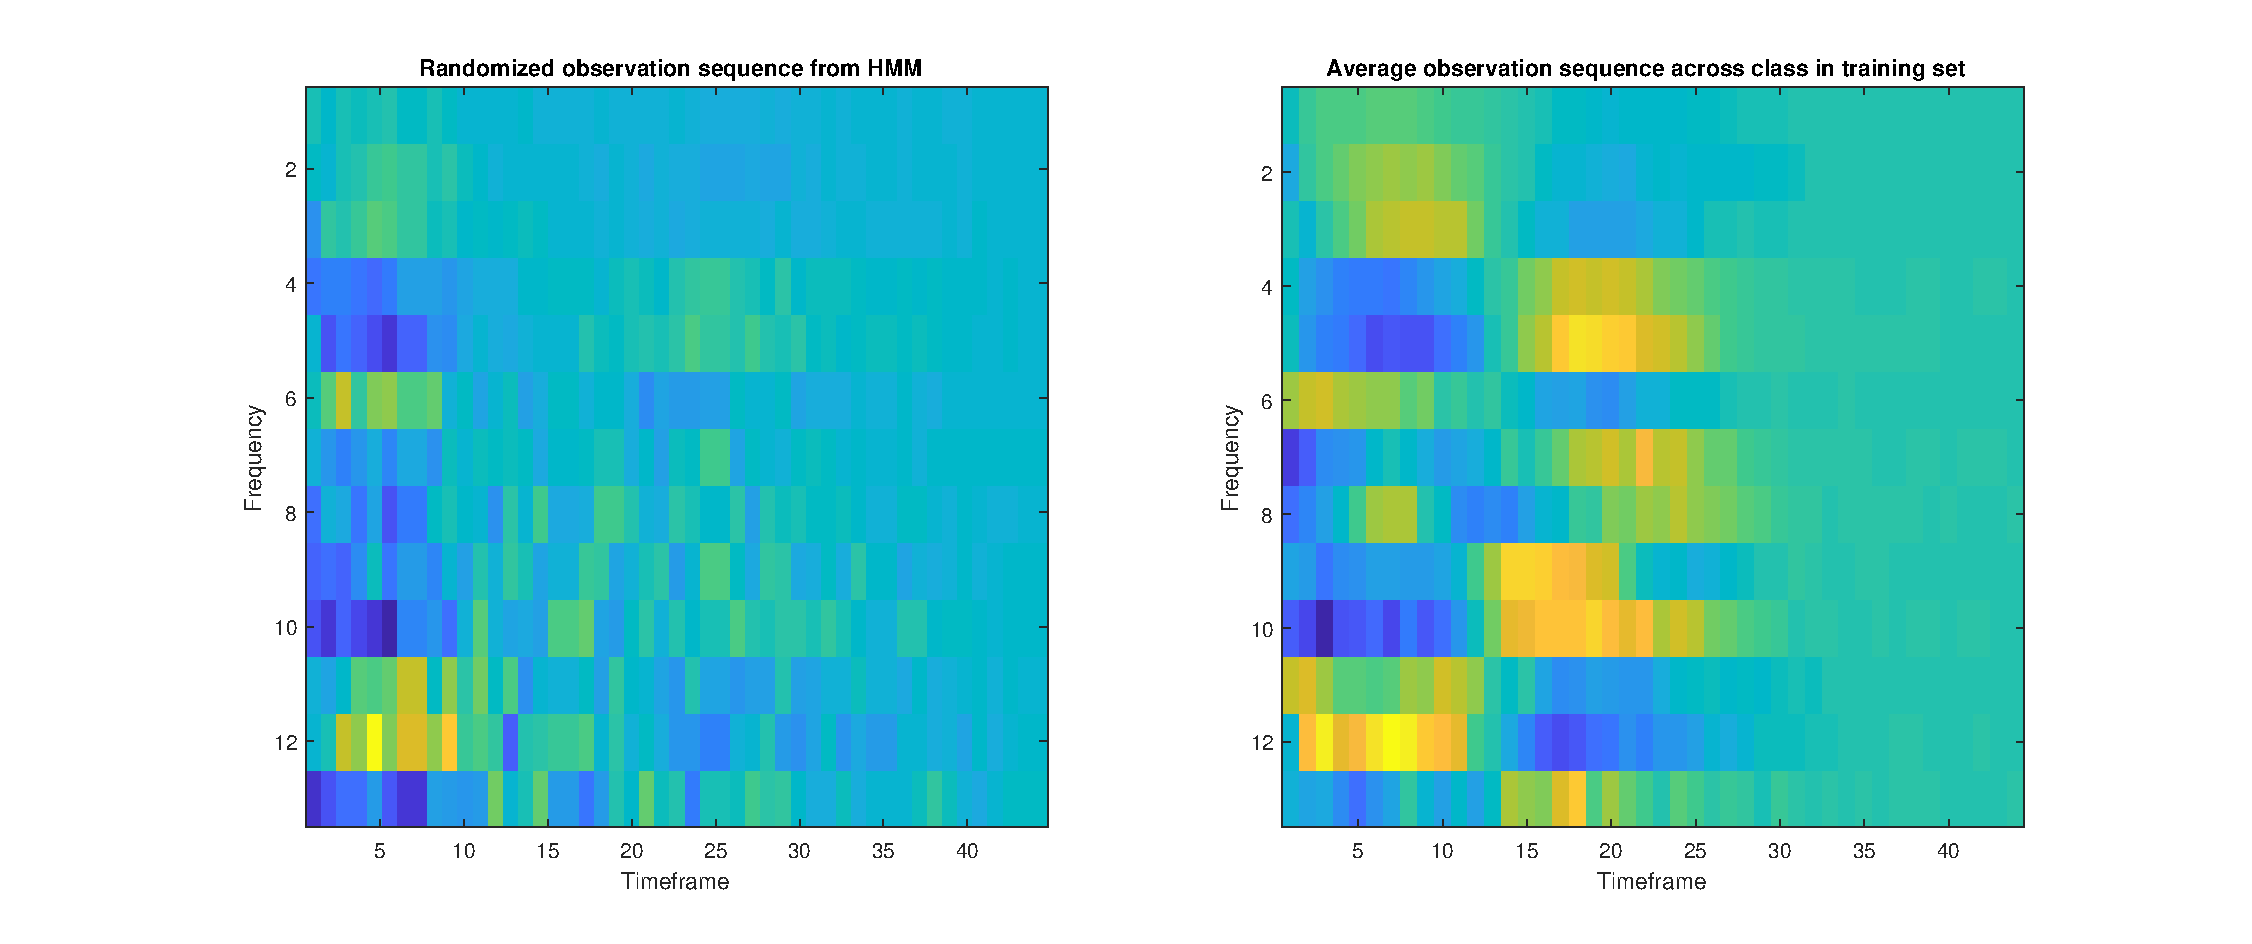
\includegraphics{../Results/randCompClass4.eps}
\caption{Randomized vs training data class four}
\end{figure}

\begin{figure}
\centering
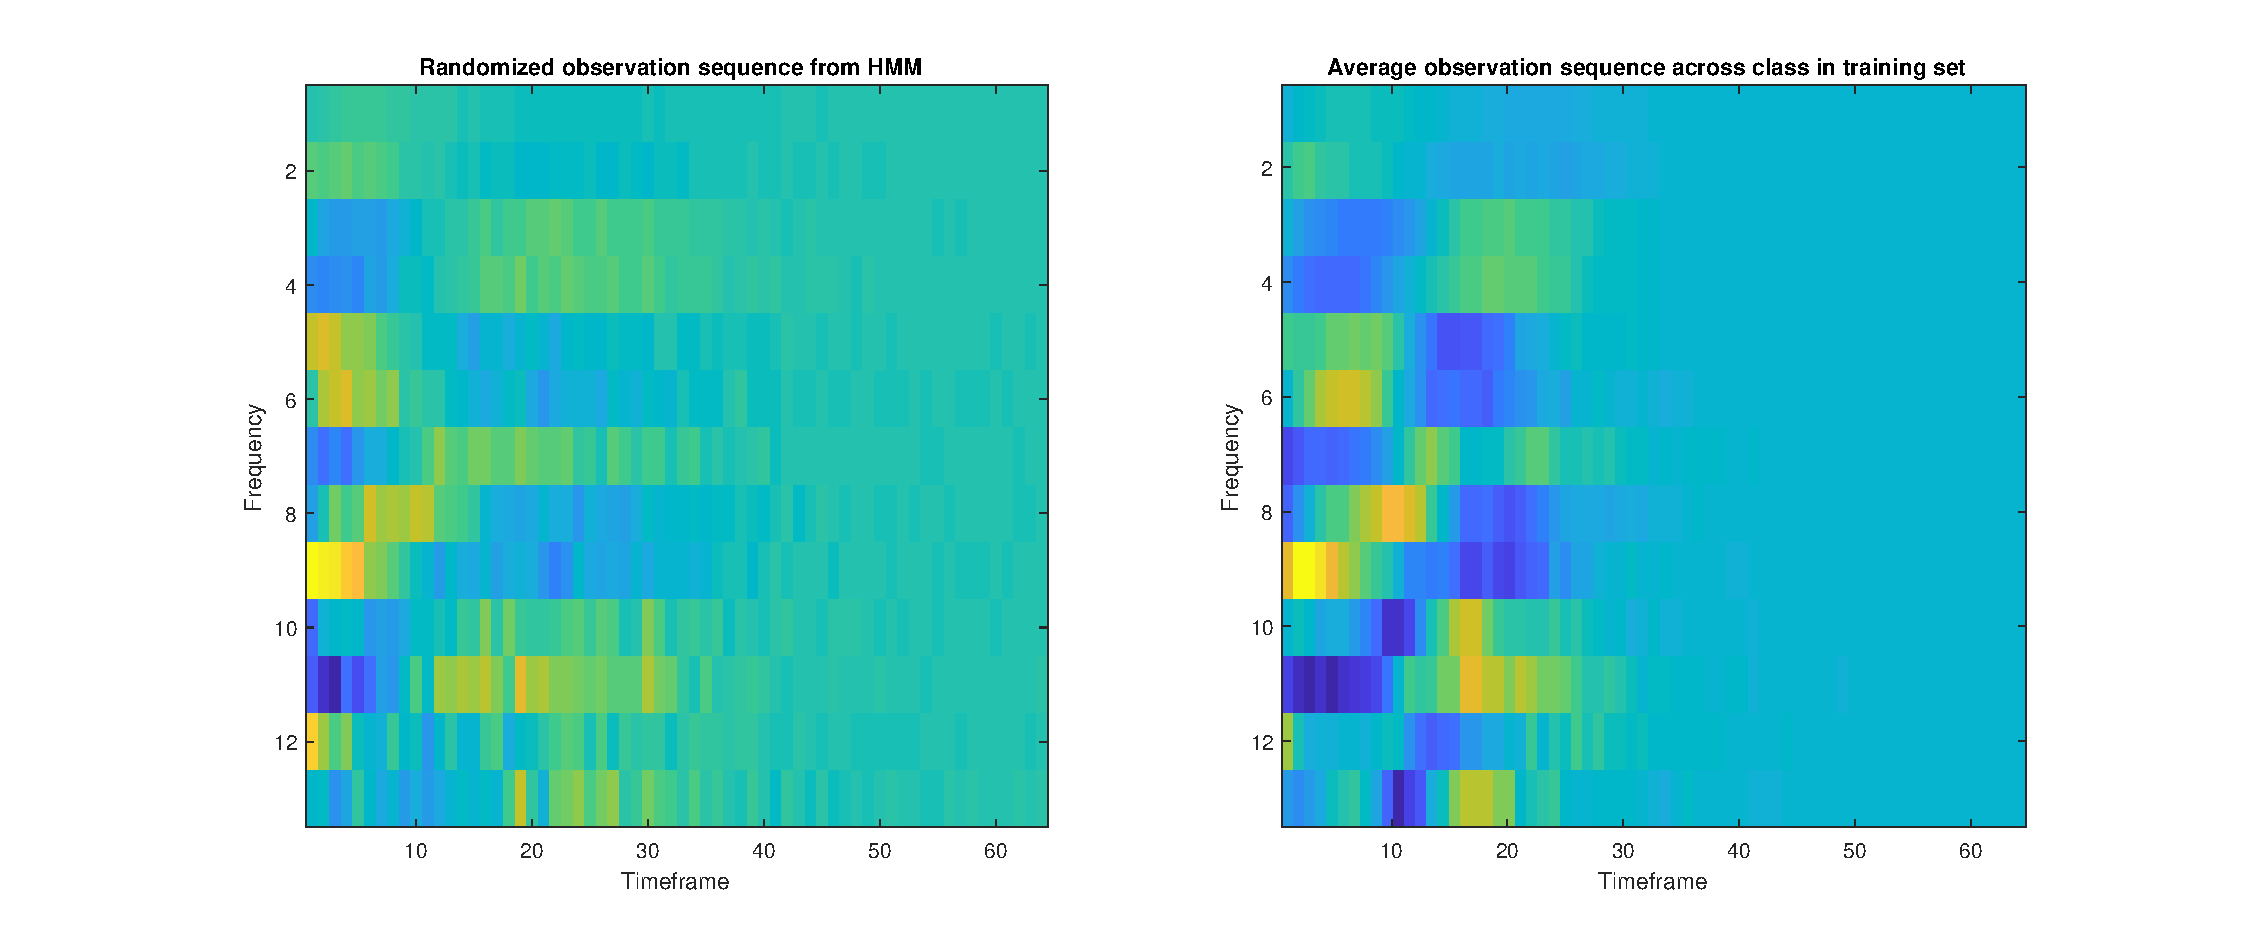
\includegraphics{../Results/randCompClass5.eps}
\caption{Randomized vs training data class five}
\end{figure}

\begin{figure}
\centering
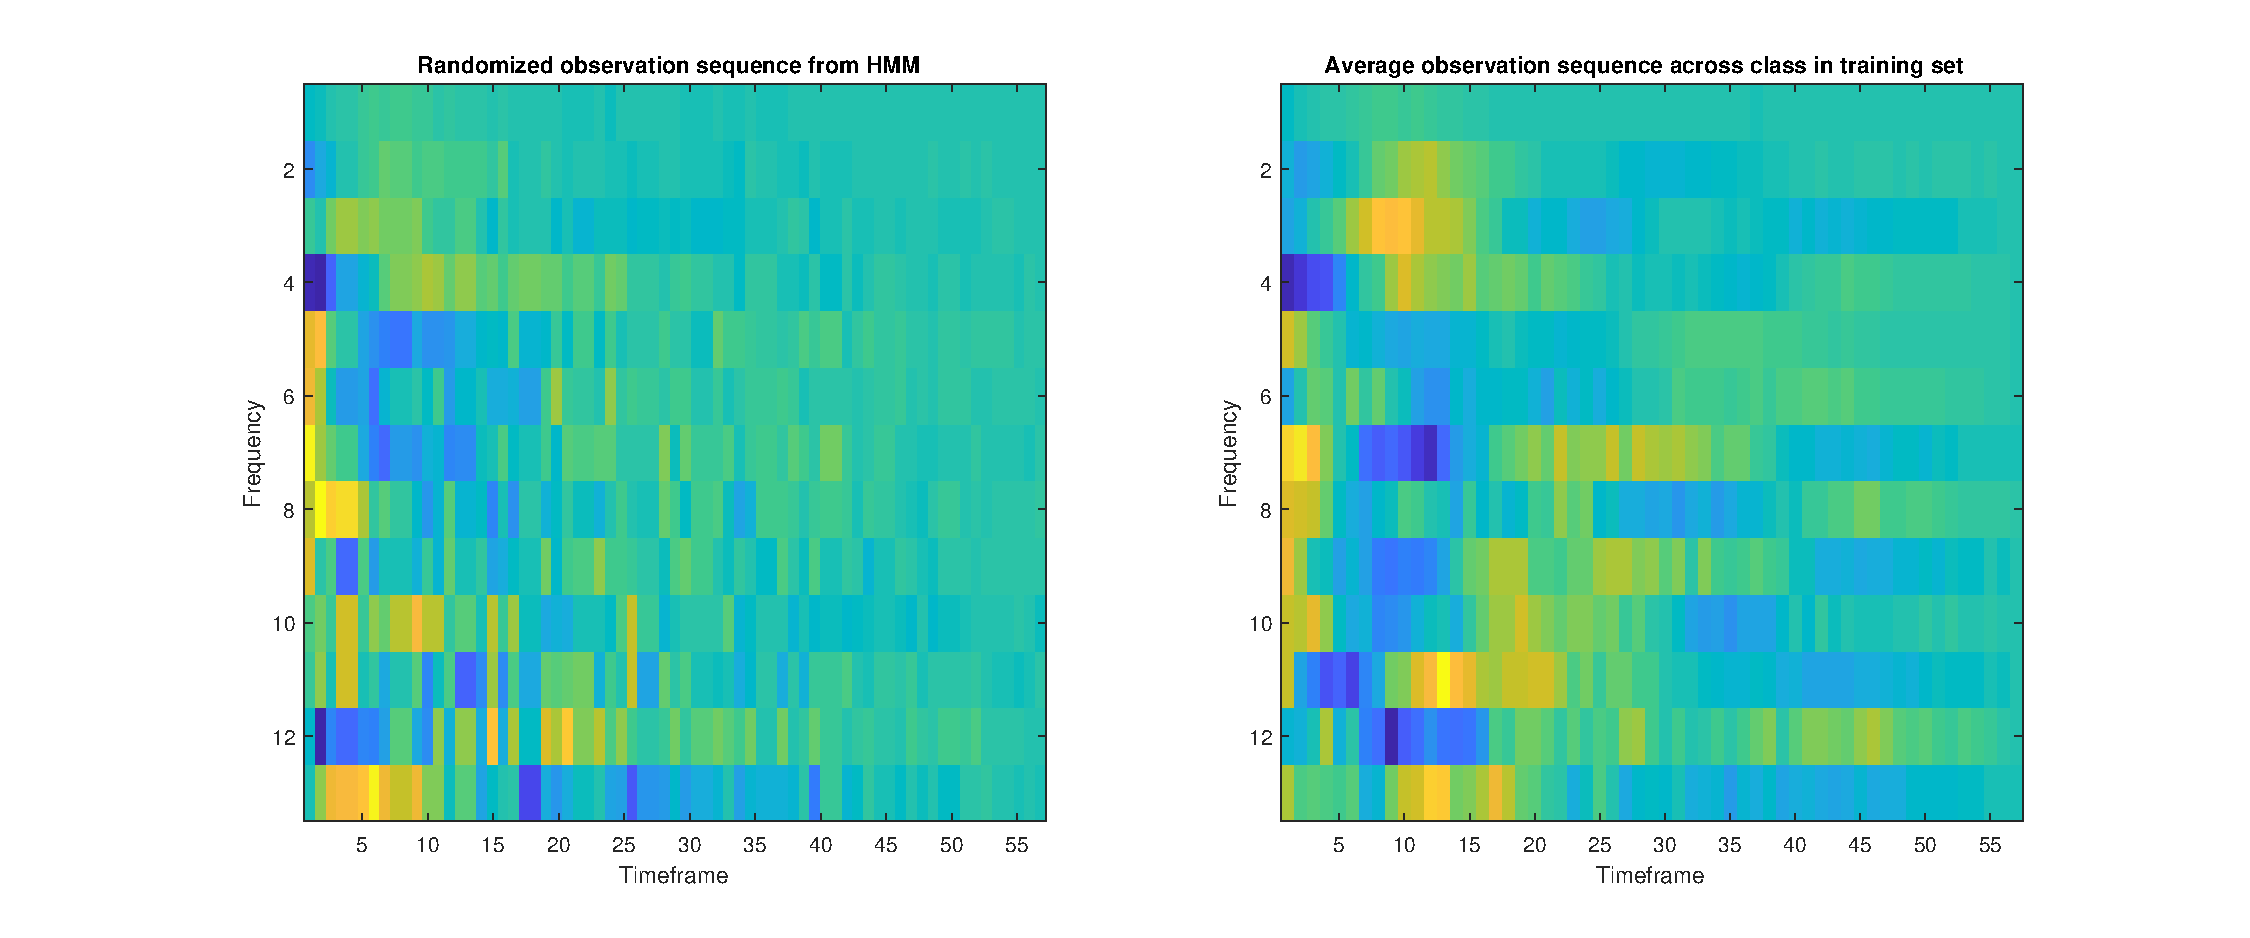
\includegraphics{../Results/randCompClass6.eps}
\caption{Randomized vs training data class six}
\end{figure}

\begin{figure}
\centering
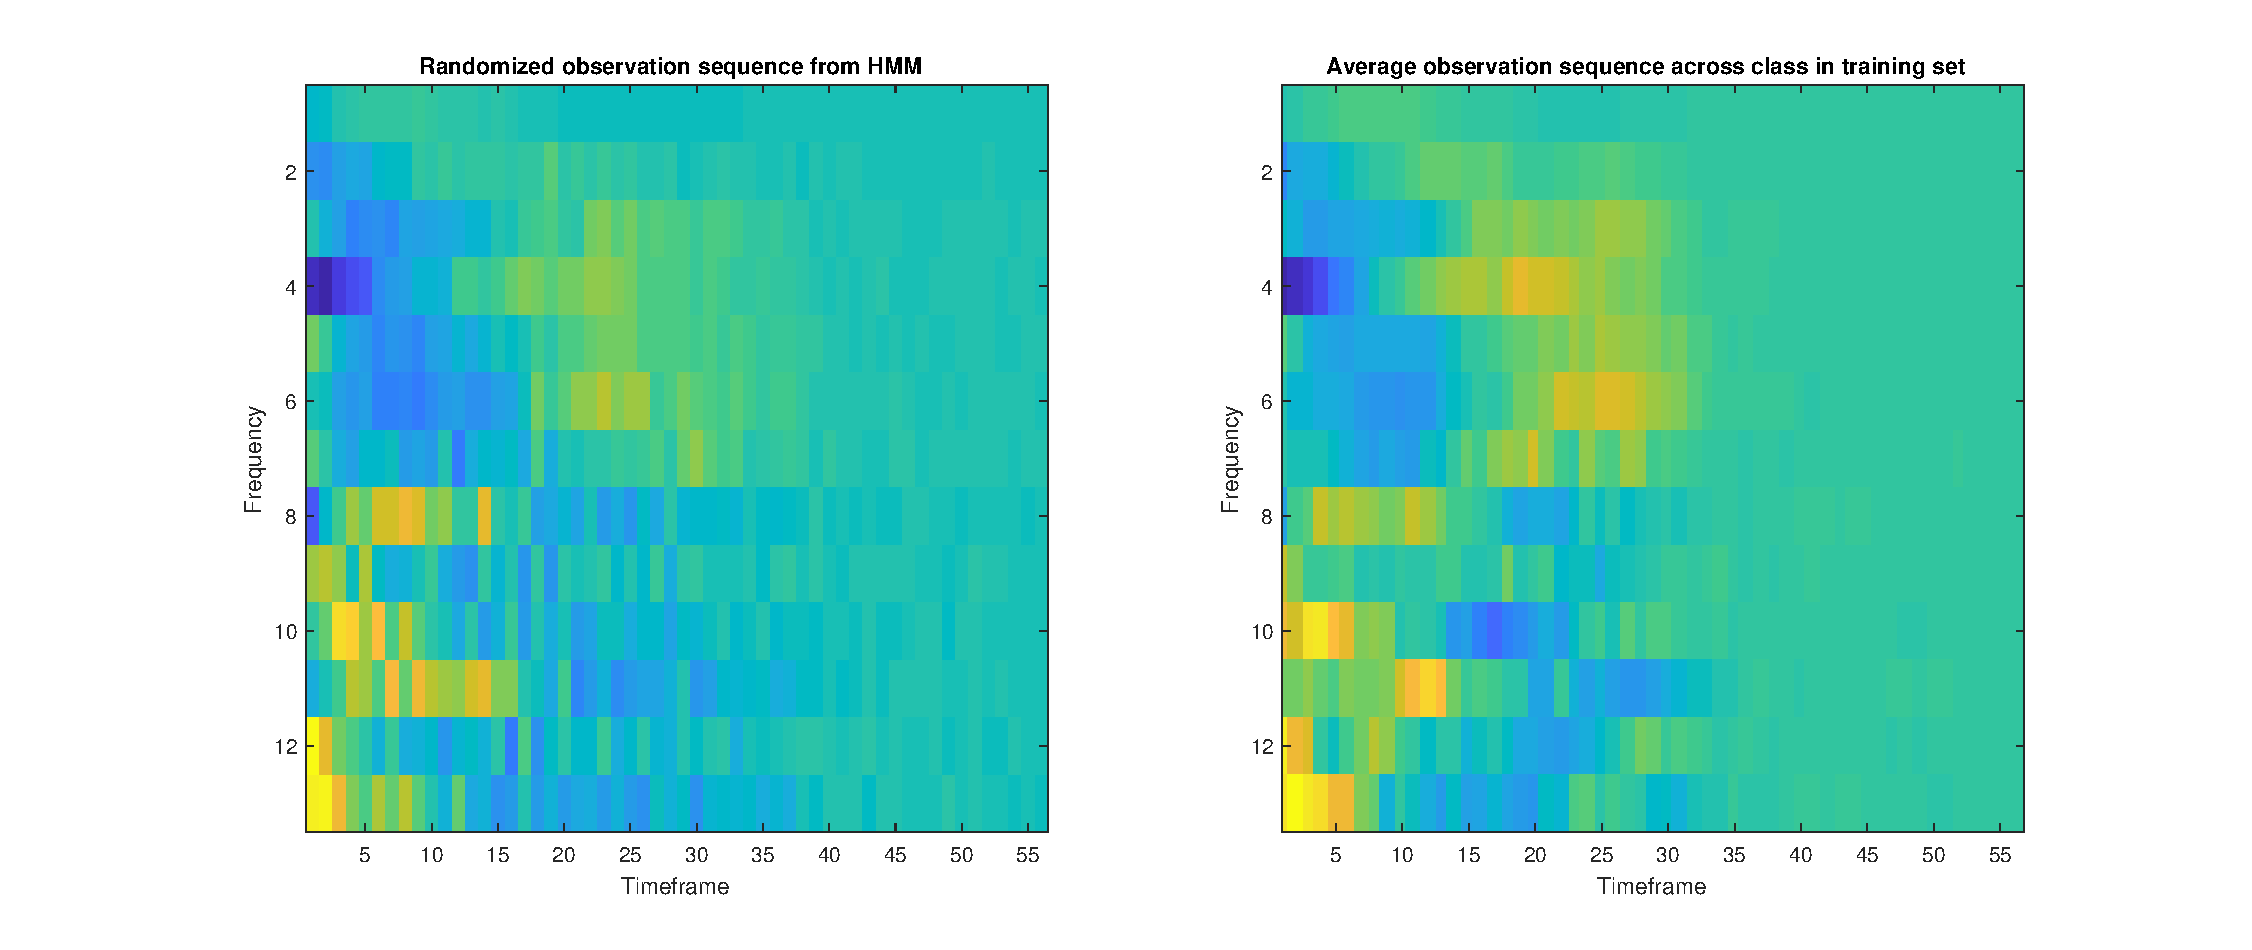
\includegraphics{../Results/randCompClass7.eps}
\caption{Randomized vs training data class seven}
\end{figure}

\begin{figure}
\centering
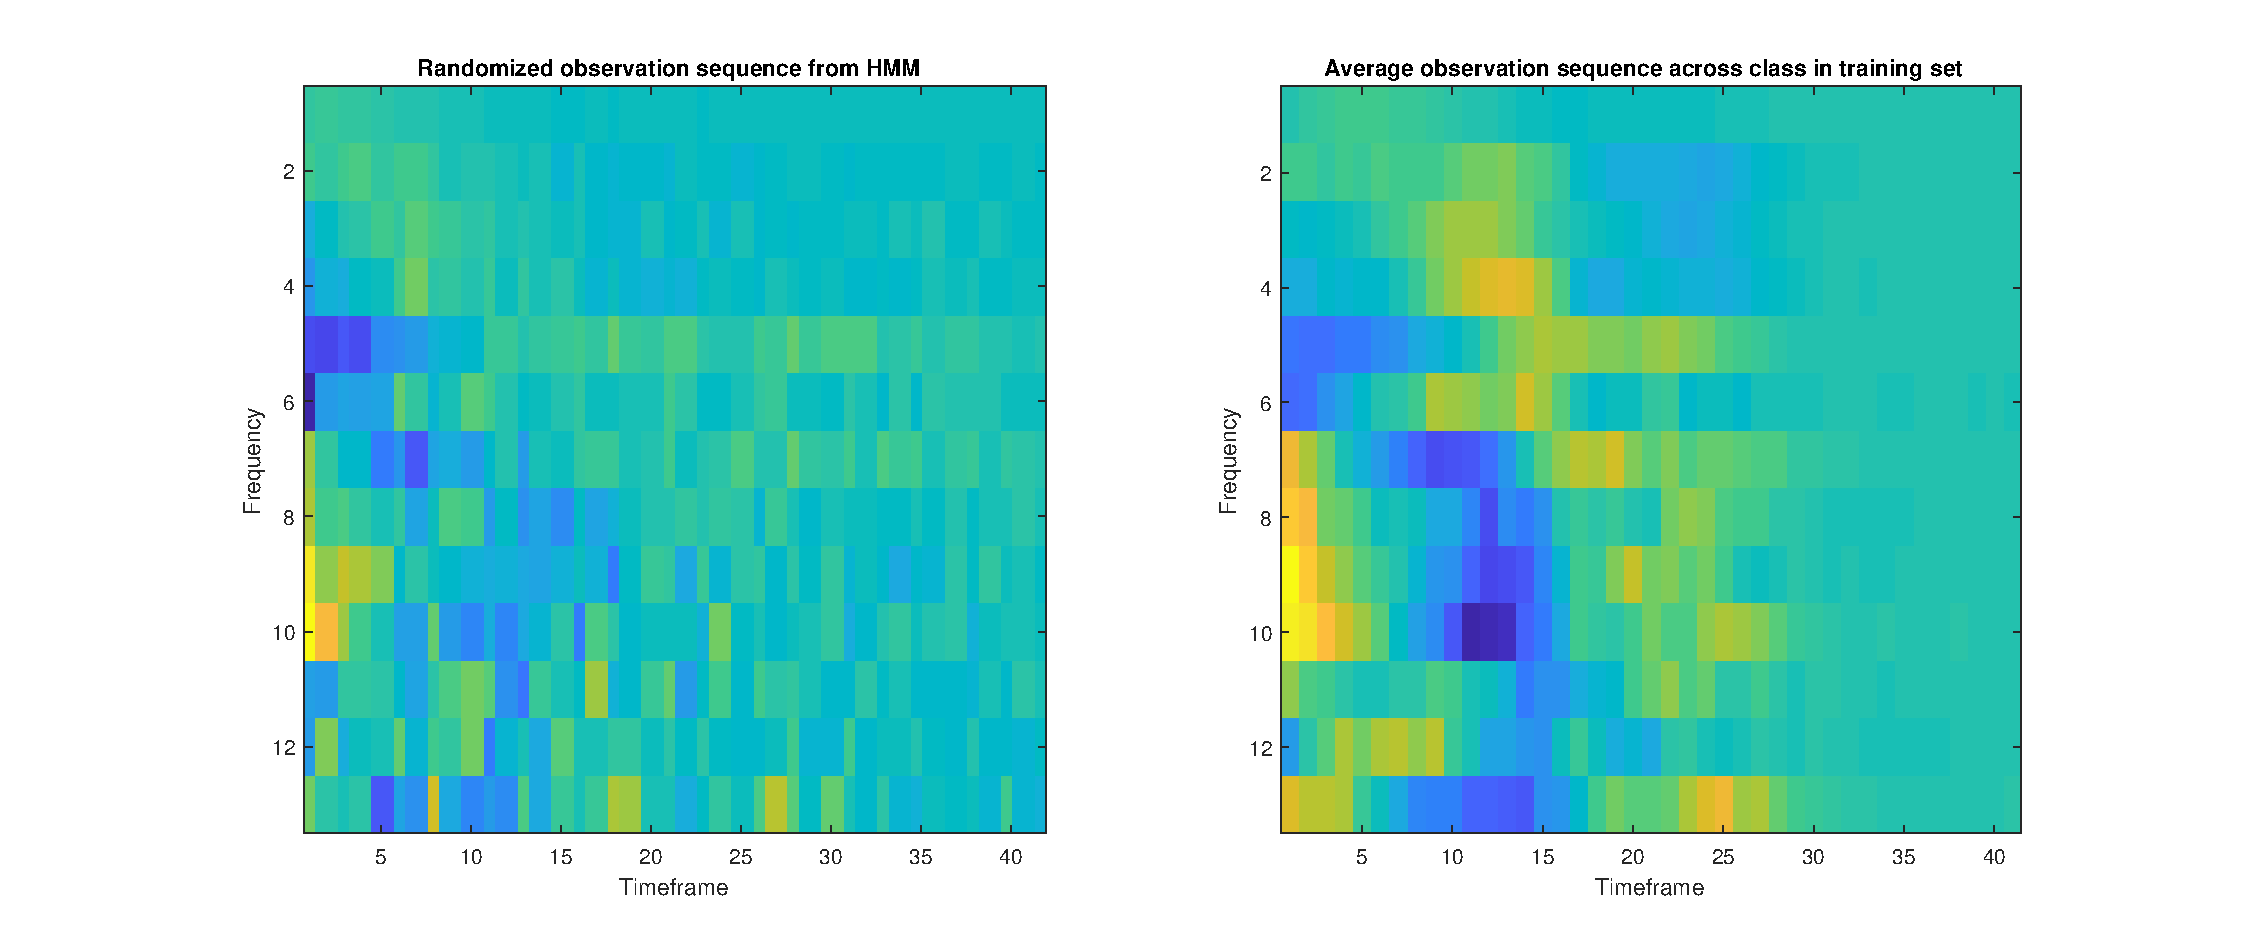
\includegraphics{../Results/randCompClass8.eps}
\caption{Randomized vs training data class eight}
\end{figure}

\begin{figure}
\centering
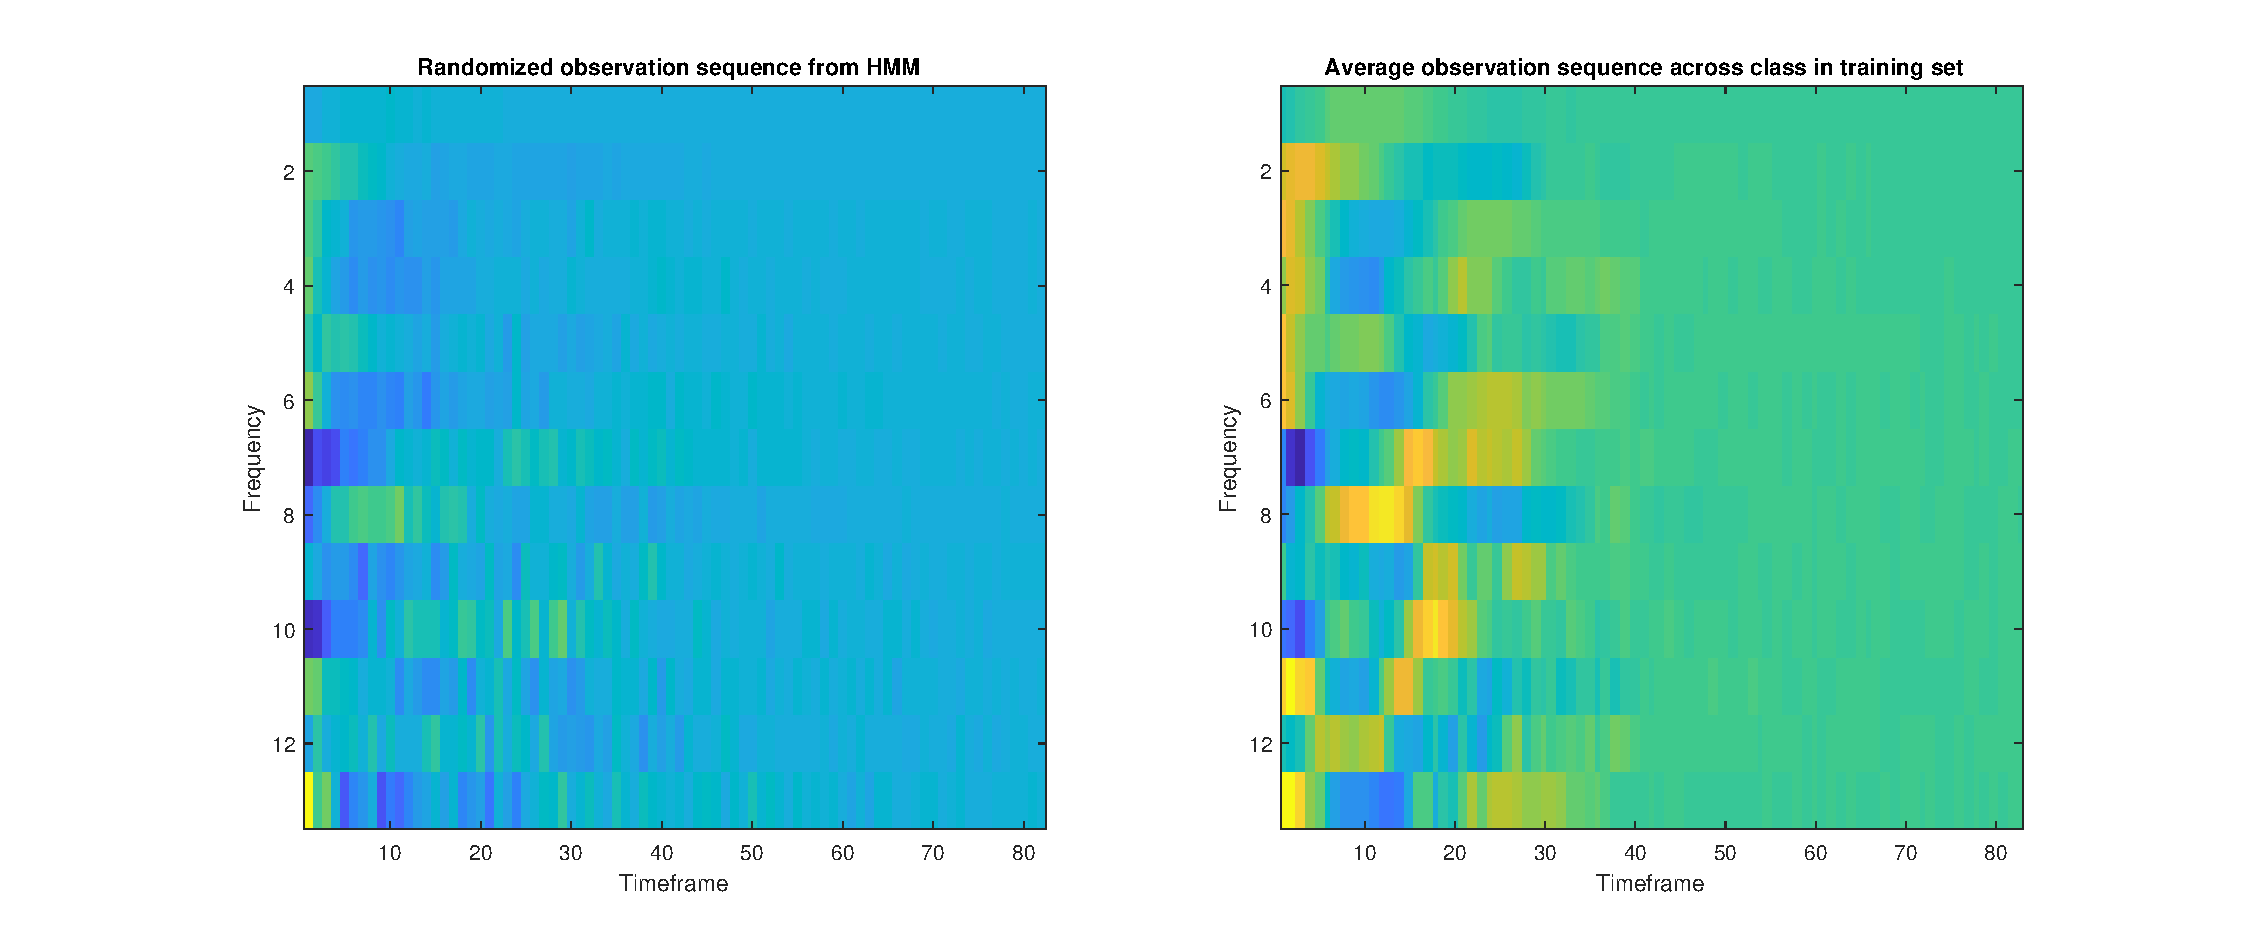
\includegraphics{../Results/randCompClass9.eps}
\caption{Randomized vs training data class nine}
\end{figure}

\newpage

\hypertarget{missclassified-instances}{%
\section{Missclassified instances}\label{missclassified-instances}}

Some missclassified examples can be seen below:

\begin{figure}
\centering
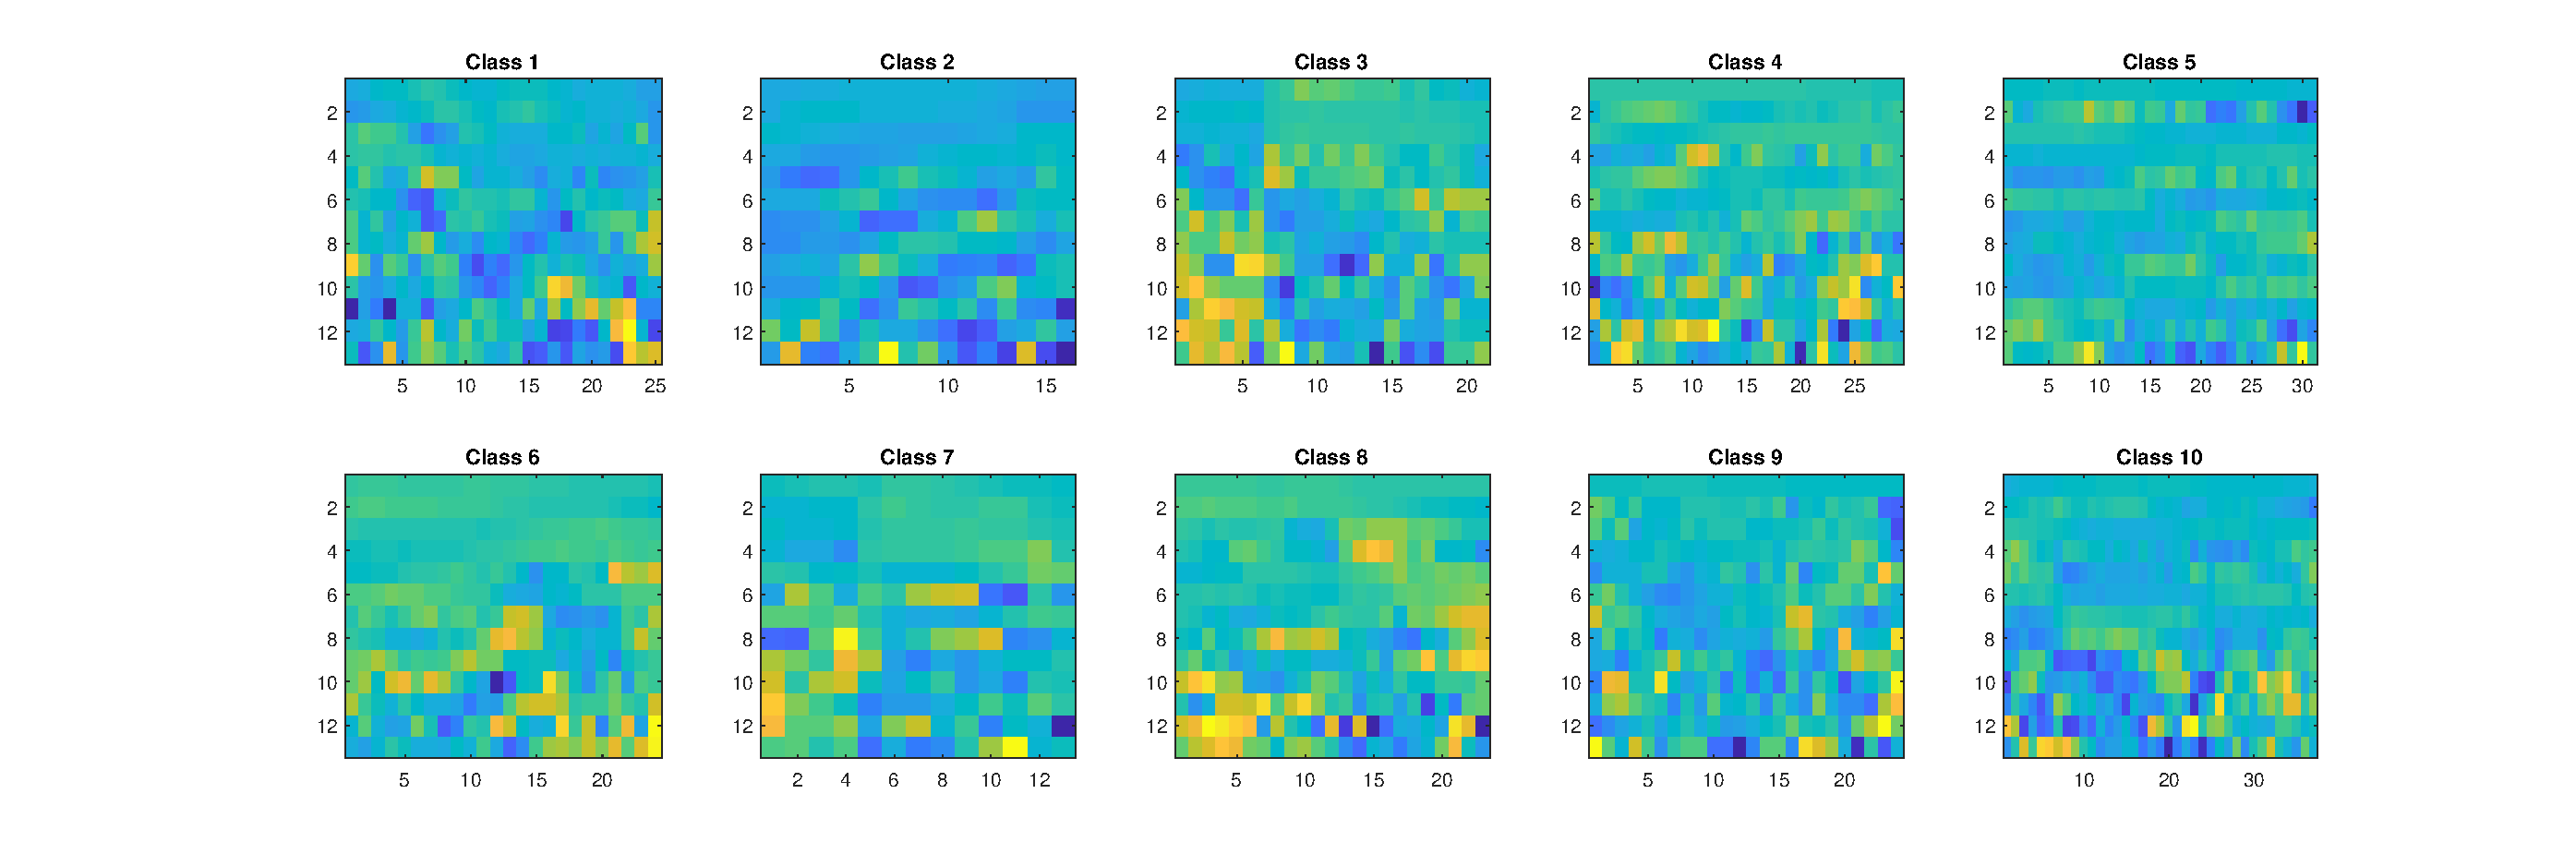
\includegraphics{../Results/missclassifiedInstances.eps}
\caption{Example missclassified instances}
\end{figure}

\hypertarget{confusion-matrix}{%
\section{Confusion matrix}\label{confusion-matrix}}

The confusion matrix took the following form:

\begin{figure}
\centering
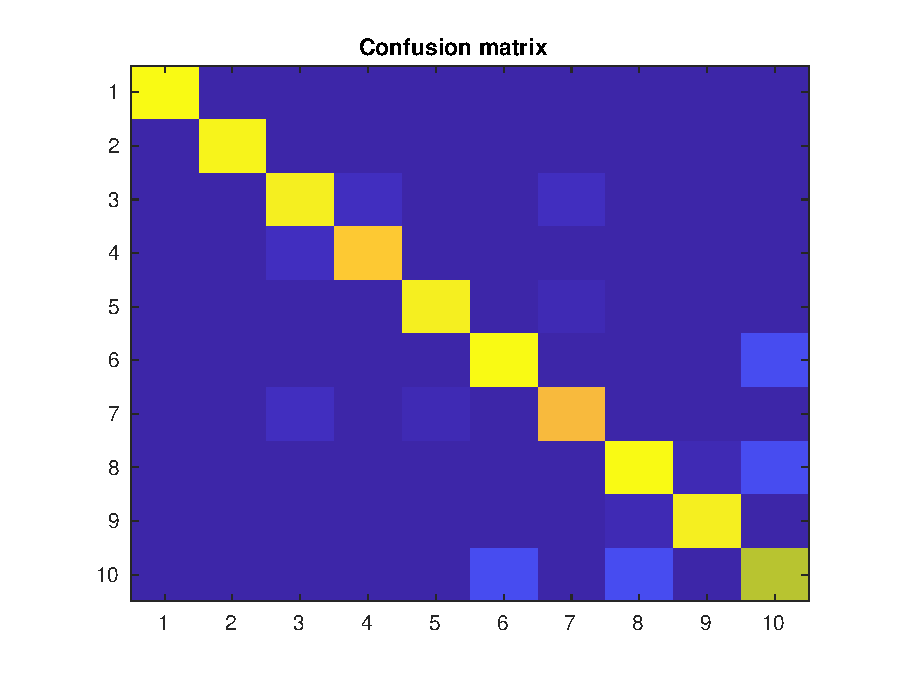
\includegraphics{../Results/confusionMatrix.eps}
\caption{Confusion matrix}
\end{figure}

\hypertarget{live-demo}{%
\section{Live demo}\label{live-demo}}

Did not work at all when trained on the given dataset. But we created
our own dataset, and trained a new model which worked significantly
better\ldots{}

\hypertarget{conclusions}{%
\section{Conclusions}\label{conclusions}}

\begin{itemize}
\item
  Though we had a rather large dataset with 4 speakers and 50 recordings
  per class (a total of 2 000). It still was not enough to generalize to
  our voices.
\item
  Variablilty in pronouciation can lead to different amounts or outright
  different phonmemes, leading to issues when trying to generalize.
\end{itemize}


\end{document}
